\documentclass[11pt,a4paper]{article}

\usepackage{amsfonts,amssymb,amsmath}
\usepackage[margin=1in]{geometry}
\usepackage[none]{hyphenat}
\usepackage{graphicx}
\usepackage{fancyhdr}
\usepackage{float}
\usepackage{color}
\usepackage{xcolor}
\usepackage{tikz}
\usepackage[nottoc,notlot,notlof]{tocbibind}

\usetikzlibrary{arrows.meta,patterns,shapes}

\parindent 0ex
\setlength{\parskip}{0.55\baselineskip}
\setlength{\abovedisplayskip}{0.5\baselineskip}
\setlength{\belowdisplayskip}{0.5\baselineskip}
\setlength{\abovedisplayshortskip}{0.25\baselineskip}
\setlength{\belowdisplayshortskip}{0.25\baselineskip}
\numberwithin{equation}{section}

\pagestyle{fancy}
\fancyfoot[C]{\thepage}
\fancyhead{}
\fancyhead[R]{\rightmark}
\renewcommand{\headrulewidth}{0pt}

% Upright operator names; plain italic would read Var as the product V.a.r.
\DeclareMathOperator{\Var}{Var}
\DeclareMathOperator{\Cov}{Cov}
\DeclareMathOperator{\OR}{OR}
\DeclareMathOperator{\RR}{RR}
\DeclareMathOperator{\RD}{RD}

% Theorem environments.
\usepackage{amsthm}
\theoremstyle{definition}
% One shared counter running section.subsection.n, as in the other courses here.
\newtheorem{thm}{Theorem}[subsection]
\newtheorem{defn}[thm]{Definition}
\newtheorem{exa}[thm]{Example}
\newtheorem{prop}[thm]{Proposition}
\newtheorem{coro}[thm]{Corollary}
\newtheorem{lem}[thm]{Lemma}
\newtheorem{result}[thm]{Result}
\newtheorem{exe}[thm]{Exercise}
\newtheorem*{note}{Note}
\newtheorem*{remark}{Remark}
\newtheorem{problemx}{Problem}[subsection]
\newenvironment{problem}{\begin{problemx}}{\end{problemx}}
\newenvironment{solution}
  {\renewcommand{\qedsymbol}{}\begin{proof}[\textit{Solution}.]}
  {\end{proof}}
\usepackage{enumitem}
% A heading that is legal inside a theorem body, a list or a float, where
% \subsubsection is not. Same weight as \subsubsection* so the two read alike.
\newcommand{\subhead}[1]{%
  \par\medskip\noindent\textbf{#1}\par\nobreak\smallskip}

\begin{document}
% Title page depersonalised for the web, as with every other course here. The
% identity kept below is the invariance of the odds ratio, the reason a
% case-control study can answer a question asked about risks.
\begin{titlepage}
\thispagestyle{empty}
\begin{center}
\vspace*{3cm}
{\Huge\bfseries Statistics in Epidemiology}\\[1.2cm]
{\large Lecture Notes}\\[2.5cm]
\line(1,0){300}\\[1.5cm]
$$\frac{P(E \mid D)\,/\,P(\bar E \mid D)}{P(E \mid \bar D)\,/\,P(\bar E \mid \bar D)} = \frac{P(D \mid E)\,/\,P(\bar D \mid E)}{P(D \mid \bar E)\,/\,P(\bar D \mid \bar E)}$$
\end{center}
\end{titlepage}

\tableofcontents
\thispagestyle{empty}
\clearpage
\setcounter{page}{1}

\section{Introduction to epidemiological studies}
\label{sec:intro}

\subsection{What epidemiology studies}

\begin{defn}
\textbf{Epidemiology} is the study of the distribution and the determinants of health-related states and events in
specified populations, and the application of that study to the control of health problems.
\end{defn}

Three words in the definition carry the subject. \emph{Distribution} asks who becomes ill, where and when; answering it is \textbf{descriptive
epidemiology}. \emph{Determinants} asks why: which exposures, behaviours, genes or circumstances change the chance of becoming ill. Answering
it is \textbf{analytic epidemiology}, and almost all of this course is about it. \emph{Populations} says the unit of interest is a group, not a
patient. A clinician asks whether this patient has the disease; an epidemiologist asks how often the disease occurs in a group and whether
it occurs more often in one group than another.

The word \textbf{exposure} is used for any characteristic whose effect on disease is being studied: a drug, an occupation, smoking, a gene,
a water supply. The \textbf{outcome} is usually the occurrence of a disease or death, coded $D$ (disease) and $\bar D$ (no disease); exposure
is coded $E$ and $\bar E$. Both may be more than two-valued, but the binary case carries every idea and is used throughout.

The statistical problems of the subject come from the fact that in most epidemiological work the investigator cannot assign the exposure.
Nobody can be told to smoke for twenty years or to drink from a contaminated well. The data are \emph{observational}: people chose, or
were given by circumstance, their exposures, and whatever led them to it may also affect their disease. Separating the effect of the
exposure from the effects of everything that travels with it is the central task, and the methods of the later sections (standardisation,
stratification, the Mantel--Haenszel procedure, regression) are all tools for it.

\begin{exa}[Snow and the London water companies]
\label{exa:snow}
In 1854 two companies supplied water to the same districts of south London, their pipes running down the same streets. The Southwark and
Vauxhall Company drew its water from the Thames below the sewage outfalls; the Lambeth Company had moved its intake upstream. John Snow
counted cholera deaths in the first seven weeks of the epidemic by the company supplying each house, and the deaths per
$10{,}000$ houses:
\begin{center}
\begin{tabular}{lrrr}
\hline
Supply & Houses & Deaths & Per $10{,}000$ houses \\
\hline
Southwark and Vauxhall & $40{,}046$ & $1{,}263$ & $315$ \\
Lambeth & $26{,}107$ & $98$ & $38$ \\
\hline
\end{tabular}
\end{center}
The death rate in houses supplied by Southwark and Vauxhall was
\[
\frac{1263/40046}{98/26107} = \frac{0.03154}{0.00375} = 8.4
\]
times that in houses supplied by Lambeth.

Snow's argument for causation did not rest on the size of the ratio alone. He pointed out that the two supplies were intermixed house by
house, so that the customers of the two companies were alike in wealth, occupation, crowding and every other respect he could think of,
and differed only in their water. In modern language the comparison was \emph{exchangeable} (Section~\ref{sec:causation}): a natural
experiment in which circumstance had assigned the exposure almost at random. The table also shows the first data problem of the
subject. The denominator is houses, not people, because houses were what Snow could count; a rate per person, or per person-week at
risk, would need the number of residents, which he did not have.
\end{exa}

\subsection{Disease occurrence in populations}
\label{sec:occurrence}

\subhead{Populations and time}

Disease occurs in people over time, and every measure in the course has a population and a period attached. A \textbf{closed} population
(a \textbf{cohort}) gains no members after it is defined: the people enrolled in a trial, the children born in one hospital in 2010, the
workers employed at a plant on a given date. It loses members only by death or by the event studied. An \textbf{open} population, such as
the residents of a city, gains members by birth and immigration and loses them by death and emigration; individuals enter and leave
throughout the period of observation.

A person is \textbf{at risk} of a disease while they are free of it and capable of getting it. Women who have had a hysterectomy are not at
risk of uterine cancer; a child immune after measles is not at risk of measles. The population at risk is the right denominator for every
measure of how often a disease begins.

\subhead{The natural history of disease}

For a chronic disease the sequence is: exposure begins; after an \textbf{induction period} the disease process starts; after a
\textbf{latent period} it becomes detectable, then symptomatic, and is diagnosed; it ends in recovery, chronic illness or death. The
epidemiologist usually sees only the date of diagnosis. Two consequences recur. Exposure measured shortly before diagnosis may be the wrong
exposure, because the relevant one acted years earlier; and a disease that is present but not yet diagnosed makes a person look disease-free
when they are not.

\subhead{Three measures of occurrence}

There are three basic ways of saying how often a disease occurs, studied fully in a later section. Here they are introduced
informally, because the study designs differ in which of them they can estimate.

\begin{enumerate}
\item The \textbf{risk} (cumulative incidence) of a disease over a period is the probability that a person at risk at the start develops it
during the period. It is a proportion, between $0$ and $1$, and means nothing without the length of the period: the five-year risk is larger
than the one-year risk.
\item The \textbf{rate} (incidence rate, incidence density) is the number of new cases divided by the total \emph{person-time} at risk:
cases per person-year. It has units of $\text{time}^{-1}$ and can exceed one.
\item The \textbf{odds} of disease is $p/(1-p)$, where $p$ is a risk. It carries the same information as the risk but behaves better
mathematically, and it is what a case-control study can compare.
\end{enumerate}

The \textbf{prevalence} of a disease is different from all three: it is the proportion of a population that \emph{has} the disease at a
given time, counting old cases as well as new ones. Prevalence mixes how often a disease begins with how long it lasts.

\subhead{The fourfold table}

When both exposure and disease are binary, the data of almost any study can be laid out as a $2 \times 2$ table. The notation below is
used throughout the course.
\begin{center}
\begin{tabular}{l|cc|c}
 & Exposed $E$ & Unexposed $\bar E$ & Total \\
\hline
Diseased $D$ & $a$ & $b$ & $m_1$ \\
Not diseased $\bar D$ & $c$ & $d$ & $m_0$ \\
\hline
Total & $n_1$ & $n_0$ & $n$ \\
\end{tabular}
\end{center}
The columns are exposure groups and the rows are disease groups. Association is measured by:
\begin{itemize}
\item the \textbf{risk ratio} (relative risk) $\RR = \dfrac{a/n_1}{b/n_0}$;
\item the \textbf{risk difference} $\RD = \dfrac{a}{n_1} - \dfrac{b}{n_0}$;
\item the \textbf{odds ratio} $\OR = \dfrac{a/c}{b/d} = \dfrac{ad}{bc}$.
\end{itemize}
Whether these sample quantities estimate anything depends on how the table was obtained, which is the subject of the next two subsections.

\subsection{Types of epidemiological study}
\label{sec:designs}

Studies are classified first by whether the investigator assigns the exposure, then by how the subjects are selected and in which
direction in time they are followed (Figure~\ref{fig:designs}).

% The four designs as panels, in the infographic style used elsewhere in the
% notes: what each starts from, which way it looks in time, what it estimates.
% One picture, so the panels stay side by side on the web.
\begin{figure}[H]
\centering
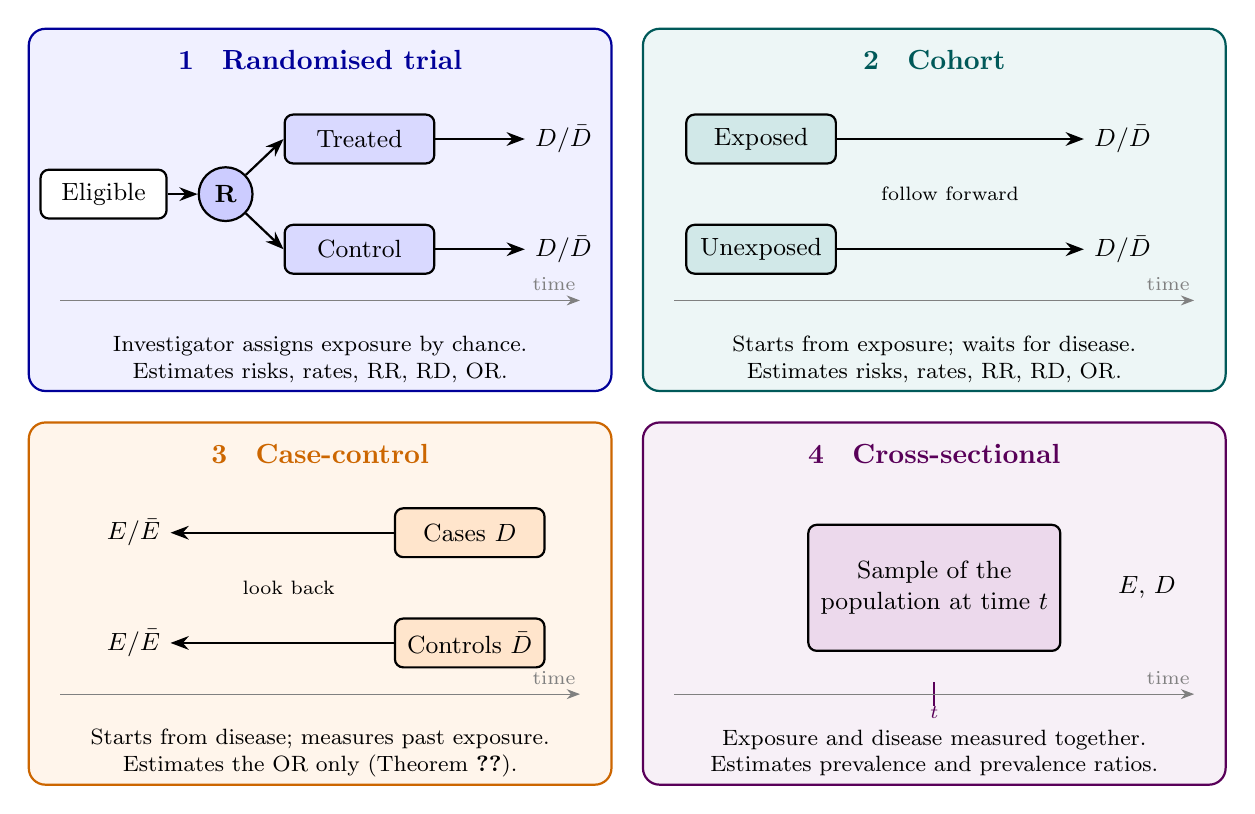
\begin{tikzpicture}[scale=1,
  box/.style={draw,thick,rounded corners=3pt,minimum width=1.9cm,minimum height=0.62cm,align=center,font=\small},
  ttl/.style={font=\bfseries},
  txt/.style={font=\footnotesize,align=center,text width=6.6cm}]
% Panel 1: randomised trial
\begin{scope}[shift={(0,0)}]
\fill[blue!6,rounded corners=6pt] (0,0) rectangle (7.4,4.6);
\draw[blue!60!black,thick,rounded corners=6pt] (0,0) rectangle (7.4,4.6);
\node[ttl,blue!60!black] at (3.7,4.2) {1\;\; Randomised trial};
\node[box,fill=white,minimum width=1.6cm] (el) at (0.95,2.5) {Eligible};
\node[circle,draw,thick,fill=blue!20,font=\small\bfseries] (r) at (2.5,2.5) {R};
\node[box,fill=blue!15] (t) at (4.2,3.2) {Treated};
\node[box,fill=blue!15] (c) at (4.2,1.8) {Control};
\draw[-Stealth,thick] (el) -- (r);
\draw[-Stealth,thick] (r) -- (t.west);
\draw[-Stealth,thick] (r) -- (c.west);
\draw[-Stealth,thick] (t.east) -- (6.3,3.2) node[right,font=\small] {$D/\bar D$};
\draw[-Stealth,thick] (c.east) -- (6.3,1.8) node[right,font=\small] {$D/\bar D$};
\draw[-Stealth,gray] (0.4,1.15) -- (7.0,1.15) node[pos=0.95,above,font=\scriptsize] {time};
\node[txt] at (3.7,0.4) {Investigator assigns exposure by chance.\\Estimates risks, rates, RR, RD, OR.};
\end{scope}
% Panel 2: cohort
\begin{scope}[shift={(7.8,0)}]
\fill[teal!7,rounded corners=6pt] (0,0) rectangle (7.4,4.6);
\draw[teal!70!black,thick,rounded corners=6pt] (0,0) rectangle (7.4,4.6);
\node[ttl,teal!70!black] at (3.7,4.2) {2\;\; Cohort};
\node[box,fill=teal!18] (e) at (1.5,3.2) {Exposed};
\node[box,fill=teal!18] (u) at (1.5,1.8) {Unexposed};
\draw[-Stealth,thick] (e.east) -- (5.6,3.2) node[right,font=\small] {$D/\bar D$};
\draw[-Stealth,thick] (u.east) -- (5.6,1.8) node[right,font=\small] {$D/\bar D$};
\node[font=\scriptsize,align=center] at (3.9,2.5) {follow forward};
\draw[-Stealth,gray] (0.4,1.15) -- (7.0,1.15) node[pos=0.95,above,font=\scriptsize] {time};
\node[txt] at (3.7,0.4) {Starts from exposure; waits for disease.\\Estimates risks, rates, RR, RD, OR.};
\end{scope}
% Panel 3: case-control
\begin{scope}[shift={(0,-5.0)}]
\fill[orange!8,rounded corners=6pt] (0,0) rectangle (7.4,4.6);
\draw[orange!80!black,thick,rounded corners=6pt] (0,0) rectangle (7.4,4.6);
\node[ttl,orange!80!black] at (3.7,4.2) {3\;\; Case-control};
\node[box,fill=orange!20] (ca) at (5.6,3.2) {Cases $D$};
\node[box,fill=orange!20] (co) at (5.6,1.8) {Controls $\bar D$};
\draw[-Stealth,thick] (ca.west) -- (1.8,3.2) node[left,font=\small] {$E/\bar E$};
\draw[-Stealth,thick] (co.west) -- (1.8,1.8) node[left,font=\small] {$E/\bar E$};
\node[font=\scriptsize,align=center] at (3.3,2.5) {look back};
\draw[-Stealth,gray] (0.4,1.15) -- (7.0,1.15) node[pos=0.95,above,font=\scriptsize] {time};
\node[txt] at (3.7,0.4) {Starts from disease; measures past exposure.\\Estimates the OR only (Theorem~\ref{thm:orinv}).};
\end{scope}
% Panel 4: cross-sectional
\begin{scope}[shift={(7.8,-5.0)}]
\fill[violet!6,rounded corners=6pt] (0,0) rectangle (7.4,4.6);
\draw[violet!70!black,thick,rounded corners=6pt] (0,0) rectangle (7.4,4.6);
\node[ttl,violet!70!black] at (3.7,4.2) {4\;\; Cross-sectional};
\node[box,fill=violet!15,minimum width=3.2cm,minimum height=1.6cm] at (3.7,2.5) {Sample of the\\population at time $t$};
\node[font=\small] at (6.4,2.5) {$E$, $D$};
\draw[violet!70!black,thick] (3.7,1.0) -- (3.7,1.3) node[below=5pt,font=\scriptsize] {$t$};
\draw[-Stealth,gray] (0.4,1.15) -- (7.0,1.15) node[pos=0.95,above,font=\scriptsize] {time};
\node[txt] at (3.7,0.4) {Exposure and disease measured together.\\Estimates prevalence and prevalence ratios.};
\end{scope}
\end{tikzpicture}
\caption{The four basic designs. Arrows show the direction in which each design moves through time: a trial and a cohort study go
from exposure to disease, a case-control study from disease back to exposure, and a cross-sectional study takes one snapshot.}
\label{fig:designs}
\end{figure}

\subhead{Experimental studies}

In a \textbf{randomised controlled trial} the investigator assigns the exposure (usually a treatment) by a chance mechanism and follows the
groups to compare outcomes. Randomisation makes the groups comparable, in distribution, in every characteristic measured or not, which is
why the trial is the standard against which observational designs are judged. A \textbf{field trial} randomises healthy people to a
preventive measure (a vaccine, a dietary supplement); a \textbf{community trial} randomises whole communities (fluoridation of water,
a health-education campaign). Trials are possible only for exposures that are expected to do good, or at least no harm; nobody may be
randomised to asbestos.

\subhead{Cohort studies}

A \textbf{cohort study} identifies exposed and unexposed people who are free of the disease and follows them over time to record who
develops it. It may be \textbf{prospective} (follow-up runs from now into the future) or \textbf{historical} (retrospective): exposure is
reconstructed from past records, such as employment files, and follow-up from then to now is done through death registers. In either case
the logical direction is from exposure to disease. Cohort studies measure risks and rates directly, can study many diseases after one
exposure, and establish that exposure came before disease. They are expensive and slow for rare diseases: to see $50$ cases of a disease with
annual rate $10^{-4}$ needs half a million person-years.

\subhead{Case-control studies}

A \textbf{case-control study} starts at the other end. It collects people with the disease (\textbf{cases}) and a sample of people without
it (\textbf{controls}) from the population that produced the cases, then compares their histories of exposure. It is fast and cheap for rare
diseases, which is why most of what is known about the causes of cancer first came from case-control studies. Its weaknesses are that
exposure is often recalled after diagnosis, when cases may remember differently from controls, and that choosing controls who truly
represent the source population of the cases is difficult. As Section~\ref{sec:estimable} shows, it cannot estimate risks, only odds ratios.

\subhead{Cross-sectional and ecological studies}

A \textbf{cross-sectional} study, also called a prevalence study, records exposure and disease in a sample of a population at one time. It
estimates prevalence and is the natural design for planning health services. Because it counts existing cases, it confuses the causes
of getting a disease with the causes of having it for a long time, and it often cannot tell whether exposure came first.

An \textbf{ecological} study uses groups, not individuals, as the unit of analysis: countries, districts, years. It relates the disease
rate of each group to the average exposure of the group, for instance the lung cancer rate of each country to its cigarette consumption per
head. The data are cheap, often already published, but associations between groups need not hold for the individuals in them
(Example~\ref{exa:ecological}).

\subsection{What each design can estimate}
\label{sec:estimable}

The designs differ statistically in which margins of the $2 \times 2$ table are fixed by the investigator. Let the population
probabilities be
\[
p_1 = P(D \mid E), \qquad p_0 = P(D \mid \bar E), \qquad q_1 = P(E \mid D), \qquad q_0 = P(E \mid \bar D),
\]
so that $p_1, p_0$ are the risks in the exposed and unexposed, and $q_1, q_0$ are the probabilities of exposure among the diseased and
non-diseased.

\begin{prop}[Sampling models]
\label{prop:sampling}
Under random sampling within the groups fixed by the design:
\begin{enumerate}
\item \emph{Cross-sectional}: only $n$ is fixed, and $(a, b, c, d)$ is multinomial with cell probabilities $P(D \cap E)$, \dots.
Every probability in the table can be estimated.
\item \emph{Cohort}: $n_1$ and $n_0$ are fixed and $a \sim \text{Bin}(n_1, p_1)$, $b \sim \text{Bin}(n_0, p_0)$ independently. The risks $p_1, p_0$ and every
function of them are estimable; $q_1, q_0$ are not, since they depend on the proportion exposed, which the investigator chose.
\item \emph{Case-control}: $m_1$ and $m_0$ are fixed and $a \sim \text{Bin}(m_1, q_1)$, $c \sim \text{Bin}(m_0, q_0)$ independently. The exposure
probabilities $q_1, q_0$ are estimable; $p_1, p_0$ are not, since they depend on the proportion diseased, which the investigator chose.
\end{enumerate}
\end{prop}

\begin{proof}
In the cohort design the $n_1$ exposed subjects are a random sample from the exposed population, so each one independently has the
disease with probability $p_1$; likewise for the unexposed. In the case-control design each sampled case is exposed with probability
$q_1$ and each control with probability $q_0$. To see that the risks cannot be estimated in a case-control study, use Bayes' theorem
with $\pi = P(D)$:
\[
p_1 = \frac{q_1 \pi}{q_1 \pi + q_0 (1 - \pi)},
\]
which takes every value in $(0,1)$ as $\pi$ ranges over $(0,1)$ with $q_1, q_0$ fixed. The distribution of the data depends only on $(q_1, q_0)$,
so two populations with the same $(q_1, q_0)$ but different $\pi$ give the same distribution of data and different $p_1$. No function of the data
can be consistent for $p_1$. The cohort argument is the same with the roles of $E$ and $D$ exchanged.
\end{proof}

So the case-control study, which samples on disease, cannot estimate the risk ratio, which is the quantity of interest. What rescues it is
the following identity, which is why the odds ratio is everywhere in epidemiology.

\begin{thm}[Invariance of the odds ratio]
\label{thm:orinv}
The \emph{exposure odds ratio} among the diseased and non-diseased equals the \emph{disease odds ratio} among the exposed and unexposed:
\[
\frac{q_1/(1 - q_1)}{q_0/(1 - q_0)} = \frac{p_1/(1 - p_1)}{p_0/(1 - p_0)} .
\]
\end{thm}

\begin{proof}
Both sides equal the cross-product ratio of the joint probabilities. Write $\pi_{DE} = P(D \cap E)$ and similarly for the other three cells.
Then $q_1 = \pi_{DE}/P(D)$ and $1 - q_1 = \pi_{D\bar E}/P(D)$, so $q_1/(1 - q_1) = \pi_{DE}/\pi_{D\bar E}$; similarly $q_0/(1 - q_0) = \pi_{\bar D E}/\pi_{\bar D \bar E}$. The
left side is therefore
\[
\frac{\pi_{DE}\,\pi_{\bar D \bar E}}{\pi_{D\bar E}\,\pi_{\bar D E}} .
\]
On the right, $p_1/(1 - p_1) = \pi_{DE}/\pi_{\bar D E}$ and $p_0/(1 - p_0) = \pi_{D\bar E}/\pi_{\bar D \bar E}$, whose ratio is the same cross-product.
\end{proof}

\begin{coro}
In a case-control study the sample odds ratio $ad/(bc)$ estimates the disease odds ratio $\OR = p_1(1 - p_0)/\{p_0(1 - p_1)\}$ of the source
population, consistently as $m_1, m_0 \to \infty$.
\end{coro}

\begin{proof}
$a/m_1 \to q_1$ and $c/m_0 \to q_0$ in probability by the law of large numbers, and $b/m_1 \to 1 - q_1$, $d/m_0 \to 1 - q_0$. The sample odds ratio
$ad/(bc) = \{(a/m_1)(d/m_0)\}/\{(b/m_1)(c/m_0)\}$ is a continuous function of these four, so it converges to the exposure odds ratio, which equals the
disease odds ratio by Theorem~\ref{thm:orinv}.
\end{proof}

When the disease is rare in both exposure groups the odds ratio is close to the risk ratio, since
\[
\OR = \RR \cdot \frac{1 - p_0}{1 - p_1}
\]
and the second factor is near $1$ when $p_0$ and $p_1$ are both small. This \textbf{rare disease assumption} is what lets a case-control
study of cancer be read as estimating a relative risk. A later section shows that with a suitable choice of controls
(\emph{density sampling}) the odds ratio estimates the \emph{rate} ratio exactly, without the assumption.

\begin{exa}[Same exposure probabilities, different risk ratios]
Suppose in two populations $q_1 = P(E \mid D) = 0.6$ and $q_0 = P(E \mid \bar D) = 0.3$, so a case-control study in either gives the same
data in distribution. The odds ratio is $(0.6/0.4)/(0.3/0.7) = 3.5$ in both. If the disease has prevalence $\pi = 0.01$ in the first
population, Bayes' theorem gives $p_1 = 0.0198$ and $p_0 = 0.0057$, and $\RR = 3.45$, close to the odds ratio. If $\pi = 0.2$ in the
second, then $p_1 = 0.333$, $p_0 = 0.125$, and $\RR = 2.67$. The case-control data cannot tell these populations apart; the odds ratio is the
part of the association they can recover.
\end{exa}

\begin{prop}[Case-control study with known sampling fractions]
\label{prop:fractions}
If cases are sampled from the source population with known probability $f_1$ and non-cases with known probability $f_0$, then the
number of exposed cases in the source population is estimated by $a/f_1$ and of exposed non-cases by $c/f_0$, and
\[
\hat p_1 = \frac{a/f_1}{a/f_1 + c/f_0}, \qquad \hat p_0 = \frac{b/f_1}{b/f_1 + d/f_0}
\]
estimate the risks. Their ratio $\hat p_1/\hat p_0$ estimates the risk ratio, and their odds ratio is $ad/(bc)$ whatever $f_1, f_0$.
\end{prop}

\begin{proof}
Each exposed case in the population is included with probability $f_1$, so $E(a) = f_1 N_{DE}$, where $N_{DE}$ is the number of exposed cases;
$a/f_1$ is unbiased for $N_{DE}$ and $c/f_0$ for $N_{\bar D E}$. The risk among the exposed is $N_{DE}/(N_{DE} + N_{\bar D E})$, estimated by substituting.
For the odds ratio, $\hat p_1/(1 - \hat p_1) = (a/f_1)/(c/f_0)$ and $\hat p_0/(1 - \hat p_0) = (b/f_1)/(d/f_0)$; the sampling fractions cancel in the ratio.
\end{proof}

\begin{exa}
A registry records all $200$ cases of a disease in a town over a year, so $f_1 = 1$. A random $1\%$ of the town's non-cases is sampled as
controls, $f_0 = 0.01$. Of the cases $120$ were exposed and $80$ not; of $300$ controls $90$ were exposed and $210$ not. The estimated numbers
of exposed and unexposed non-cases in the town are $9000$ and $21{,}000$, so
\[
\hat p_1 = \frac{120}{120 + 9000} = 0.0132, \qquad \hat p_0 = \frac{80}{80 + 21000} = 0.0038,
\]
so $\widehat{\RR} = 0.0132/0.0038 = 3.47$,
while the odds ratio is $(120 \times 210)/(80 \times 90) = 3.50$. A population-based case-control study with known sampling fractions is
a cohort study in which only a sample of the non-cases has been measured.
\end{exa}

\subsection{Association and causation}
\label{sec:causation}

An association between exposure and disease, however strong, is not by itself evidence that the exposure causes the disease. To say
precisely what causation would mean, imagine each person's outcome under each exposure.

\begin{defn}[Potential outcomes]
For each person let $Y^1$ be the disease indicator that would be observed if the person were exposed and $Y^0$ the indicator if unexposed.
The exposure has a \textbf{causal effect} on a person if $Y^1 \neq Y^0$. In a population the \textbf{causal risk ratio} and \textbf{causal risk difference} are
\[
\frac{P(Y^1 = 1)}{P(Y^0 = 1)} \qquad\text{and}\qquad P(Y^1 = 1) - P(Y^0 = 1) ,
\]
comparing the risk if everyone were exposed with the risk if no one were.
\end{defn}

Only one of $Y^1, Y^0$ is ever seen for a given person: under \textbf{consistency}, the observed outcome is $Y = Y^1$ for the exposed and $Y = Y^0$
for the unexposed. The observed (associational) risk ratio $P(Y = 1 \mid E)/P(Y = 1 \mid \bar E)$ compares different people, and equals the causal risk
ratio only under a condition on how exposure was assigned.

\begin{defn}
Exposure is \textbf{exchangeable} with respect to the outcome if $(Y^1, Y^0)$ is independent of $E$: the exposed and unexposed would have
had the same distribution of outcomes under either exposure.
\end{defn}

\begin{thm}
\label{thm:exchange}
Under consistency and exchangeability the associational risk ratio and risk difference equal the causal ones.
\end{thm}

\begin{proof}
By consistency $P(Y = 1 \mid E) = P(Y^1 = 1 \mid E)$, and by exchangeability $P(Y^1 = 1 \mid E) = P(Y^1 = 1)$. Likewise $P(Y = 1 \mid \bar E) = P(Y^0 = 1 \mid \bar E) = P(Y^0 = 1)$.
The associational measures are therefore built from the same two numbers as the causal ones.
\end{proof}

Randomisation makes the exposure independent of everything that exists before it, including $(Y^1, Y^0)$, so a randomised trial delivers
exchangeability by design. An observational study does not, and when exchangeability fails the associational measure is said to be
\textbf{confounded}. Confounding is treated formally in a later section. The practical response, used throughout the course, is to
find variables $C$ (age, sex, social class) such that exchangeability holds \emph{within} the strata of $C$, and to compare like with
like there.

\subhead{Judging causation from observational evidence}

Because exchangeability can never be verified from observational data, causal conclusions there rest on judgement. Hill (1965) listed
aspects of an association that make a causal reading more or less plausible: its \emph{strength} (a large risk ratio is harder to explain
away by confounding), \emph{consistency} across studies and populations, \emph{specificity}, \emph{temporality} (exposure must precede
disease, the only one that is necessary), a \emph{biological gradient} (dose--response), \emph{plausibility}, \emph{coherence} with
other knowledge, \emph{experimental} evidence and \emph{analogy}. They are not criteria to be scored. Each has exceptions, and a modern
reading treats them as questions about bias: could confounding, selection or measurement error produce an association this strong, this
consistent, with this gradient?

\begin{exa}[The ecological fallacy]
\label{exa:ecological}
Three regions have the following proportions $x$ of the population exposed and annual disease risks $r$:
\begin{center}
\begin{tabular}{lccc}
\hline
Region & A & B & C \\
\hline
Proportion exposed $x$ & $0.2$ & $0.5$ & $0.8$ \\
Disease risk $r$ & $0.01$ & $0.02$ & $0.03$ \\
\hline
\end{tabular}
\end{center}
The least squares line through the three points is $r = 0.00333 + 0.0333\,x$. Read naively, a wholly unexposed region ($x = 0$) has risk
$0.00333$ and a wholly exposed one ($x = 1$) has risk $0.0367$, an \emph{ecological} risk ratio of $0.0367/0.00333 = 11$.

Now suppose that within each region the risk is the same in exposed and unexposed people: $0.01$ in A, $0.02$ in B, $0.03$ in C. The data
above are exactly what this produces, yet the exposure has no effect on anyone. The regional risks differ for some other reason that
happens to rise with the proportion exposed, such as the age structure of the regions. Group-level data cannot separate the two
explanations, because they do not record who among the exposed became ill.
\end{exa}

\begin{prop}
Let region $j$ have exposure proportion $x_j$ and risks $p_{1j}$, $p_{0j}$ among its exposed and unexposed. If $p_{1j} = p_1$ and $p_{0j} = p_0$ in every
region, then the regional risks lie exactly on the line $r = p_0 + (p_1 - p_0)x$, and the ecological risk ratio equals $p_1/p_0$.
\end{prop}

\begin{proof}
The risk in region $j$ is the average of the two group risks weighted by group size, $r_j = p_{0j}(1 - x_j) + p_{1j}\,x_j$. With common $p_1, p_0$ this is
$p_0 + (p_1 - p_0)x_j$, linear in $x_j$ with intercept $p_0$ and value $p_1$ at $x = 1$.
\end{proof}

The ecological analysis is sound when the baseline risk $p_{0j}$ does not vary with the exposure proportion, and the effect does not either. Both
are assumptions about individuals that group data cannot check. In Example~\ref{exa:ecological} $p_{0j}$ rises with $x_j$, so the
condition fails.

\subsection{Problems}

\begin{problem}
\label{prob:snow}
In Example~\ref{exa:snow}:
\begin{enumerate}[label=(\alph*)]
\item Give the risk difference in cholera deaths per $10{,}000$ houses between the two supplies, and say what it measures that the
ratio $8.4$ does not.
\item Snow's denominator is houses. State an assumption under which the ratio of deaths per house equals the ratio of deaths per
person, and give a way in which it could fail.
\end{enumerate}
\end{problem}

\begin{solution}
(a) $315.4 - 37.5 = 277.9$ deaths per $10{,}000$ houses in seven weeks. If the Southwark and Vauxhall houses had instead received
Lambeth water, and the ratio reflects the effect of the water, about $278$ deaths per $10{,}000$ houses would have been avoided. The
difference measures the burden of the exposure on an absolute scale; the ratio measures the strength of the association, which is what
bears on causation. A ratio of $8.4$ on a tiny baseline could be of little public-health importance; here both are large.

(b) Let $h_1, h_0$ be the average number of residents per house in the two groups. Deaths per person are deaths per house divided by $h_1$ or
$h_0$, so the ratio per person is $8.4 \times h_0/h_1$. The two ratios agree when $h_1 = h_0$. They would differ if, say, the cheaper company
supplied more crowded houses. Snow's argument that the supplies were intermixed street by street makes a large difference in occupancy
unlikely.
\end{solution}

\begin{problem}
Classify each study and say whether it can estimate the risk of disease in the exposed.
\begin{enumerate}[label=(\alph*)]
\item All $412$ children diagnosed with leukaemia in a country over five years are compared with $1200$ children drawn at random
from the birth register, on whether their mothers had a pelvic X-ray in pregnancy.
\item Workers employed at a smelter in 1950--1960 are identified from company records, and their deaths up to 2020 are found through the
national death index.
\item A household survey records current smoking and current chronic bronchitis in a random sample of adults.
\item Villages are randomly allocated to receive insecticide-treated bed nets or not, and malaria episodes in children are counted over
two years.
\end{enumerate}
\end{problem}

\begin{solution}
(a) A case-control study (sampling on disease). Risk is not estimable from the data alone; the odds ratio is. If the number of births in
the source population is known, the controls are a known fraction of the non-cases and Proposition~\ref{prop:fractions} recovers risks.
(b) A historical cohort study: exposure (employment) is defined at the start and deaths are followed forward from records. Risks and
rates are estimable.
(c) A cross-sectional study. It estimates the prevalence of bronchitis among smokers and non-smokers, not the risk of developing it.
(d) A community (cluster-randomised) trial. Risks and rates are estimable, with the village as the unit of randomisation, which
the analysis must take into account.
\end{solution}

\begin{problem}
Show that $\OR \geq \RR \geq 1$ when $p_1 \geq p_0$, and $\OR \leq \RR \leq 1$ when $p_1 \leq p_0$. So the odds ratio always lies further from $1$ than the
risk ratio.
\end{problem}

\begin{solution}
$\OR = \RR \cdot (1 - p_0)/(1 - p_1)$. If $p_1 \geq p_0$ then $\RR = p_1/p_0 \geq 1$ and $1 - p_0 \geq 1 - p_1$, so the second factor is at least $1$ and
$\OR \geq \RR$. If $p_1 \leq p_0$ both inequalities reverse: $\RR \leq 1$ and the factor $(1 - p_0)/(1 - p_1) \leq 1$, so $\OR \leq \RR$.
\end{solution}

\begin{problem}
\label{prob:po}
A population of eight people has the potential outcomes below.
\begin{center}
\begin{tabular}{lcccccccc}
\hline
Person & 1 & 2 & 3 & 4 & 5 & 6 & 7 & 8 \\
\hline
$Y^1$ & 1 & 1 & 1 & 0 & 1 & 0 & 0 & 0 \\
$Y^0$ & 1 & 1 & 0 & 0 & 1 & 0 & 0 & 0 \\
Exposed? & yes & yes & yes & yes & no & no & no & no \\
\hline
\end{tabular}
\end{center}
\begin{enumerate}[label=(\alph*)]
\item Find the causal risk ratio and the observed risk ratio.
\item Which people does the exposure affect? Explain the difference between the two ratios.
\end{enumerate}
\end{problem}

\begin{solution}
(a) $P(Y^1 = 1) = 4/8$ and $P(Y^0 = 1) = 3/8$, so the causal risk ratio is $4/3$. Observed: the exposed (persons 1--4) show $Y^1 = 1, 1, 1, 0$, a
risk of $3/4$; the unexposed (5--8) show $Y^0 = 1, 0, 0, 0$, a risk of $1/4$. The observed risk ratio is $3$.

(b) Only person 3 has $Y^1 \neq Y^0$; the exposure causes that person's disease. Persons 1, 2 and 5 would be ill either way. Three of the four
\emph{doomed} people (1, 2, 5) are in the exposed group, so the exposed would have had risk $2/4$ even without exposure, against $1/4$ for
the unexposed. Exchangeability fails, and the observed ratio mixes the effect of the exposure with the higher baseline risk of the
exposed: the association is confounded.
\end{solution}

\begin{problem}
Three regions have exposure proportions $0.1$, $0.4$ and $0.7$. In each region the risk is $0.02$ in the unexposed and $0.04$ in the exposed.
Find the regional risks and the ecological risk ratio, and explain why the answer is correct here but not in Example~\ref{exa:ecological}.
\end{problem}

\begin{solution}
$r_j = 0.02(1 - x_j) + 0.04x_j = 0.02 + 0.02x_j$, giving $0.022$, $0.028$ and $0.034$. These lie exactly on $r = 0.02 + 0.02x$, so the
ecological risk ratio is $(0.02 + 0.02)/0.02 = 2$, the individual risk ratio. The baseline risk is the same in every region and so is the effect,
which is the condition of the last proposition. In Example~\ref{exa:ecological} the baseline risk rose with the proportion exposed, and the
regression attributed that rise to the exposure.
\end{solution}

\begin{problem}
In a case-control study the controls are sampled from people still free of disease at the \emph{end} of the study period. Use
Theorem~\ref{thm:orinv} to say what the sample odds ratio estimates, and show that when the risks are small it approximates the risk ratio.
Find the risk ratio and the odds ratio if $p_1 = 0.02$ and $p_0 = 0.01$, and if $p_1 = 0.4$ and $p_0 = 0.2$.
\end{problem}

\begin{solution}
The controls are a sample of $\bar D$, the cases of $D$, so $a/m_1$ and $c/m_0$ estimate $q_1$ and $q_0$, and by Theorem~\ref{thm:orinv} the sample
odds ratio estimates the disease odds ratio $p_1(1 - p_0)/\{p_0(1 - p_1)\} = \RR\,(1 - p_0)/(1 - p_1)$, which tends to $\RR$ as $p_1, p_0 \to 0$.
With $p_1 = 0.02$, $p_0 = 0.01$: $\RR = 2$ and $\OR = 2 \times 0.99/0.98 = 2.02$. With $p_1 = 0.4$, $p_0 = 0.2$: $\RR = 2$ and $\OR = 2 \times 0.8/0.6 = 2.67$.
The approximation is good only for a rare disease.
\end{solution}

\section*{References}
\addcontentsline{toc}{section}{References}

\subhead{Prescribed texts}
\begin{enumerate}
\item Kahn, H. A., and Sempos, C. T. (1989), \emph{Statistical Methods in Epidemiology}, New York, Oxford University Press.
\item Kleinbaum, D. G., Kupper, L. L., and Morgenstern, H. (1982), \emph{Epidemiologic Research: Principles and Quantitative Methods}, New York,
Van Nostrand Reinhold (reprinted by Wiley).
\item Rothman, K. J., Greenland, S., and Lash, T. L. (2008), \emph{Modern Epidemiology} (3rd ed.), Philadelphia, Lippincott Williams \& Wilkins.
\item Jewell, N. P. (2003), \emph{Statistics for Epidemiology}, Boca Raton, FL, Chapman \& Hall/CRC.
\end{enumerate}

\subhead{Further reading}
\begin{enumerate}
\item Breslow, N. E., and Day, N. E. (1980), \emph{Statistical Methods in Cancer Research, Vol.~I: The Analysis of Case-Control Studies}, Lyon,
International Agency for Research on Cancer.
\item Hill, A. B. (1965), The environment and disease: association or causation? \emph{Proceedings of the Royal Society of Medicine}, 58,
295--300.
\item Snow, J. (1855), \emph{On the Mode of Communication of Cholera} (2nd ed.), London, John Churchill.
\end{enumerate}

\end{document}
